
%\twocolumn[\centering \Large \bf Creating Causal Embeddings for Question Answering \\with Minimal Supervision \par
%~\\
%
%\large \bf Anonymous EMNLP submission
%~\\
%~\\
%]

%\begin{abstract}
%A common model for question answering (QA) is that a good answer is one that is closely related to the question, where relatedness is often determined using general-purpose lexical models such as word embeddings. 
%We argue that a better approach is to look for answers that are related to the question in a {\em relevant way}, according to the information need of the question,
%%We argue that a better approach is to look for answers that are related to the question in {\em the right way} \todo{"the right way" doesn't say much... Can we say something like "in a way relevant to the type of information need, or something like that?}, 
%which may be determined through task-specific embeddings. 
%With causality as a use case, we implement this insight in three steps. First, we generate causal embeddings cost-effectively by bootstrapping cause-effect pairs extracted from free text using a small set of seed patterns. Second, we train dedicated embeddings over this data, by using task-specific contexts, i.e., the context of a cause is its effect. Finally, we extend a state-of-the-art reranking approach for QA to incorporate these causal embeddings. We evaluate the causal embedding models both \emph{directly} with a casual implication task,
%% \todo{"Word similarity" makes it sound like we do lexical similarity... Can you say something causal implication?}, 
% and \emph{indirectly}, in a downstream causal QA task using data from Yahoo! Answers. We show that explicitly modeling causality improves performance in both tasks. In the QA task our best model achieves 37.3\% P@1, significantly outperforming a strong baseline by 7.7\% (relative). 
%% ms: not sure if we should discuss the differences between the 2 tasks here; we might not have space; it might dilute the message.
%
%%
%%Question answering (QA) is a difficult task, complicated by the variety of question types represented in any given question set.  In this work we propose addressing question types individually through the use of dedicated relation embeddings, and here focus on causal relations. 
%%We train causal embeddings (as well as two other popular distributional similarity models) on causal tuples extracted from free text resources with minimal supervision, using a small set of high-precision patterns.   
%%We evaluate these causal models both \emph{directly} in terms of their ability to detect causality, and \emph{indirectly}, in terms of their utility on a causal subset of Yahoo! Answers.
%%In both tasks, we show that explicitly modeling causality significantly improves performance, and in the QA task our best model achieves 37.3\% precision at one, outperforming a strong information retrieval and lexical semantic baseline by 7.7\% (relative). 
%%Importantly, we also show that the results of these two evaluations are \emph{not} identical: a given model's performance on the direct evaluation does not necessarily transfer to the more complex, real-world QA task.  
%\end{abstract}

\chapter{Creating Causal Embeddings for Question Answering \\with Minimal Supervision \label{chapter:emnlp2016}}



%
\section{Introduction}
\label{sec-emnlp2016:introduction}
%\vspace{-2mm}

Question answering (QA), i.e., finding short answers to natural language questions, is one of the most important but challenging 
tasks on the road towards natural language understanding~\cite{Etzioni:11}. 
A common approach for QA is to prefer answers that are closely related to the question, where relatedness is often determined using lexical semantic models such as word embeddings~\cite{yih13,jansen14,fried2015higher}. 
%Many QA systems answer questions by looking for answers that are closely related to the question, often as determined with lexical semantic word embeddings~\todo{citation}.  
While appealing for its robustness to natural language variation, this one-size-fits-all approach does not take into account the wide range of distinct question types that can appear in any given question set, and that are best addressed individually~\cite{chu2004ibm,ferrucci2010building,clark2013study}.  

Given the variety of question types, we suggest that a better approach is to look for answers % which are not simply closely related to the question, 
that are related to the question \emph{through the appropriate relation}, e.g., a causal question should have a cause-effect relation with its answer.
If we adopt this view, and continue to work with embeddings as a mechanism for assessing relationship,
this raises a key question: how do we train and use task-specific embeddings cost-effectively? 
Using causality as a use case, we answer this question with a framework for producing causal word embeddings with minimal supervision, and a demonstration that such task-specific embeddings significantly benefit causal QA. 
%Adopting this view, here we propose using task-specific word embeddings that combine the robustness and versatility of word embeddings with the precision of addressing a specific question type.  
%As a use case, we focus on producing custom embeddings with minimal supervision that capture causality and that are thus directly applicable to causal QA.

%\todo{REMOVE?: One important hurdle for QA is that there isn't a single ``universal engine'' that can answer any question, but rather a collection of methods, each tailored to a specific question type (e.g., factoid, definitional, or causal).
%This has been repeatedly observed throughout QA research, in various domains
%\cite{chu2004ibm,ferrucci2010building,clark2013study}. 
%Building from this observation, this paper proposes a framework for developing specific QA solving methods, and, in particular, on the rapid bootstrapping of knowledge resources needed by these solving methods. We encode this knowledge as customized embedding vectors, and demonstrate that they can be generated with minimal supervision. As a use case, we focus on producing custom embeddings that capture \textit{causality} and that are thus directly applicable to causal QA. }

In particular, the contributions of this work are:

%{\flushleft {\bf (1)}} 
%A novel approach for question answering that uses task-specific distributional similarity models 

{\flushleft {\bf (1)}} 
A methodology for generating causal embeddings cost-effectively by bootstrapping cause-effect pairs extracted from free text using a small set of seed patterns, e.g., {\em X causes Y}. 
%We propose a method to generate knowledge resources for causal questions 
%We demonstrate that knowledge resources for causal questions can be generated by bootstrapping cause-effect pairs extracted from free text using a small set of high-precision patterns, e.g., {\em X causes Y}. 
We then train dedicated embedding (as well as two other distributional similarity) models over this data. \citet{levy2014dependency} have modified the algorithm of\citet{mikolov2013distributed} to use an arbitrary, rather than linear, context. Here we make this context task-specific, i.e., the context of a cause is its effect.
%embedding models (as well as alignment and convolutional neural network models) over this data. 
Further, to mitigate sparsity and noise, our models are bidirectional, and noise aware (by incorporating the likelihood of noise in the training process). 
%We achieve the latter by weighting the examples based on the likelihood that they are truly causal rather than simply associative. 

{\flushleft {\bf (2)}} The insight that QA benefits from task-specific embeddings. % , and a demonstration that this approach significantly improves performance. 
We implement a QA system that uses the above causal embeddings to answer questions and demonstrate that they significantly improve performance over a strong baseline. Further, we show that causal embeddings encode complementary information to vanilla embeddings, even when trained from the same knowledge resources. 

{\flushleft {\bf (3)}} An analysis of direct vs. indirect evaluations for task-specific word embeddings. 
We evaluate our causal models both  {\em directly}, in terms of measuring their capacity to rank causally-related word pairs over word pairs of other relations, as well as {\em indirectly} in the downstream causal QA task. 
%Importantly, the above knowledge acquisition process is completely independent from these evaluation tasks, e.g., the objective function of the embedding model does not include any information from the QA task, which guarantees modularity. 
In both tasks, our analysis indicates that including causal models significantly improves performance. 
However, from the direct evaluation, it is difficult to estimate which models will perform best in real-world tasks. Our analysis re-enforces recent observations about the limitations of word similarity evaluations~\cite{faruqui2016problems}: we show that they have limited coverage and may align poorly with real-world tasks.

%{\flushleft {\bf (3)}} For causal QA, we show that causal embeddings encode complementary information to vanilla embeddings, even when trained from the same knowledge resources. 

%the models that include causal embeddings perform significantly better than the models that do not. Further, for causal QA, we show that causal embeddings are complementary to vanilla embeddings, underlining the complexity of this QA task, which must simultaneously capture causality and associations driven by distributional similarity. \todo{reword? seems like we're contradicting our earlier statement...}

%{\flushleft {\bf (4)}} Finally, we show that there are discrepancies between direct and indirect evaluations, i.e., no model performs best in both tasks. Our analysis re-enforces recent observations about the limitations of narrow word similarity evaluations~\cite{faruqui2016problems}, in that they both have limited coverage, and can poorly align with real world tasks.

%
\section{Related Work}
\label{sec-emnlp2016:related work}
%\vspace{-2mm}

%QA with dedicated component
Addressing the need for %In the pursuit of %quest for building 
specialized solving methods in QA, 
Oh et. al~\citeyear{oh2013question} incorporate a dedicated causal component into their system, and note that it improves the overall performance.  However, their model is limited by the need for lexical overlap between a causal construction found in their knowledge base and the question itself.  Here, we develop a causal QA component that exploits specialized word embeddings to gain robustness to lexical variation.  
%which can model the likelihood of a causal link between two texts even when the exact lexical items were never observed together in the knowledge base.

% Embeddings in QA
There has been a vast body of work which demonstrates that word embeddings derived from distributional similarity are useful in many tasks, including question answering -- see \emph{inter alia}~\mbox{\cite{fried2015higher,yih13}}.  However, Levy and Goldberg~\citeyear{levy2015supervised} note that there are limitations on the type of semantic knowledge which is encoded in these general-purpose similarity embeddings. 
Therefore, here we build customized task-specific embeddings for causal QA.

%% Customized embeddings
Customized embeddings have been created for a variety of tasks, including semantic role labeling~\cite{fitzgerald2015semantic,woodsenddistributed}, and binary relation extraction ~\mbox{\cite{riedel2013relation}.}
%% For example, with semantic role labelling, custom embeddings have been learned for semantic frames, their arguments, and the roles of the arguments (e.g. \cite{fitzgerald2015semantic,woodsenddistributed}).  Riedel et al.~\citeyear{riedel2013relation} used distant supervision to learn embeddings for binary relations and argument pairs to perform automated database completion.  
%Like Riedel et al., we are interested in binary relations, but we train a dedicated embedding space for a single such relation, while they represent all relations in a single embeddding space.
Similar to Riedel et al., we train embeddings customized for specific relations, but we bootstrap training data using minimal supervision (i.e., a small set of patterns) rather than relying on distant supervision and large existing knowledge bases.  Additionally, while Riedel et al. represent all relations in a general embedding space, here we train a dedicated embedding space for just the causal relations. 
%\todo{remove: this is just text so that my citation doesn't fall across page boundaries, which makes latex cry}

In QA, embeddings have been customized to have question words that are close to either their answer words~\cite{bordes2014question}, or to structured knowledge base entries~\cite{yang2014joint}.  While these methods are useful for QA, they do not distinguish between different types of questions, and as such their embeddings are not specific to a given question type.

Additionally, embeddings have been customized to distinguish functional similarity from relatedness ~\cite{levy2014dependency,kielaspecializing}.
In particular, Levy and Goldberg train their embeddings by replacing the standard linear context of the target word with context derived from the syntactic dependency graph of the sentence.  For example, when given the word \emph{turing}, wheras a traditional embeddings model returns top associates containing topically related words such as \emph{non-deterministic} and \emph{finite-state}, the dependency-based model returns other tests (i.e., \emph{pauling, hotelling,} and \emph{hamming}).
In this work, we make use of this extension to arbitrary context in order to train our embeddings with contexts derived from binary causal relations.  We extract cause-effect text pairs such that the cause text becomes the \emph{target} text and the effect text serves as the \emph{context}. 

Recently, Faruqui et al.\citeyear{faruqui2016problems} discussed issues surrounding the evaluation of similarity word embeddings, including the lack of correlation between their performance on word-similarity tasks and ``downstream'' or real-world tasks like QA, text classification, etc.  As they advocate, in addition to a direct evaluation of our causal embeddings, we also evaluate them independently in a downstream QA task.  We provide the same comparison for two alternative approaches (an alignment model and a convolutional neural network model), confirming that the direct evaluation performance can be misleading without the task-specific, downstream evaluation. 

%\todo{better intro target/context} In this way, words which \emph{cause similar things} would be top-associates of each other.  

%In the search for ways to represent the semantic information encoded in words and text, there have been several methods proposed which are based on the distributional hypothesis of \todo{cite}.  The distributional hypothesis asserts that words which are semantically similar will tend to occur in similar word contexts.  One of the methods based on this hypothesis, the Skipgram algorithm \todo{cite and link}, or \texttt{word2vec}\footnote{\todo{link!}}, has been widely used for far-ranging NLP tasks.  This algorithm maps words onto high-dimensional dense vectors (embeddings) in such a way that words which are more similar to each other are closer together in the high-dimensional space.%, often measured through cosine similarity.  

%Levy and Goldberg also suggest that the traditional skipgram vectors encode broad topical similarity, and propose an extension of the algorithm which replaces the linear context of a given target word with arbitrary context.  
%While there we make use of the same  rather than topical similarity.  For example, when given the word \emph{turing}, wheras the traditional skipgram model returns top associates containing topically related words such as \emph{non-deterministic} and \emph{finite-state}, the dependency-based model returns other tests (i.e., \emph{pauling, hotelling,} and \emph{hamming}).

%While the specific implementation of Levy and Goldberg~\citeyear{levy2014dependency} uses dependency-derived contexts for training, their extension of the algorithm allows for \emph{arbitraty} contexts.  
%Additionally, though seldom used, the skipgram algorithm produces two sets of embeddings for each word, one for when the word serves as a target word and another for when the word serves as a context word.  Here, since the relation of interest is inherently directional, both sets of embeddings are meaningful, and so we make use of both -- the target vectors when a given word appears as a cause and the context vectors when that word appears as an effect.




%--Causal Patterns
With respect to extracting causal relations from text, Girju et al.~\citeyear{girju2002text} use modified Hearst patterns~\cite{hearst1992automatic} to extract a large number of potential cause-effect tuples, where both causes and effects must be nouns.
However, Cole et al.~\citeyear{cole2005lightweight} show that these nominal-based causal relations account for a relatively small percentage of all causal relations, and for this reason, \cite{yang2014multi} allow for more elaborate argument structures in their causal extraction by identifying verbs, and then following the syntactic subtree of the verbal arguments to construct their candidate causes and effects. 
Additionally, Do et al.~\citeyear{do2011minimally} observe that nouns as well as verbs can signal causality.  
We follow these intuitions in developing our causal patterns by using both nouns and verbs to signal potential participants in causal relations, and then allowing for the entire dominated structures to serve as the cause and/or effect arguments.

%Khoo did this over newspapers too


%\todo{POSSIBLY MOVE TO METHODS: 
%Khoo et al.~\citeyear{khoo1998automatic} also extract causal tuples using linguistic patterns, and in their error analysis they find that the majority of their errors of commission (i.e., %mislabelling a construction as casual) result from lexical ambiguity.  That is, several lexical constructions which can signal causality are also used in non-causal senses.  To minimize the noise %in the extracted pairs, we restrict ourselves to patterns with low ambiguity. 
%Further, inspired by bootstrapping literature~\cite{riloff1996automatically}, we rank the extracted tuples by their likelihood of being noisy using a formula driven by mutual information, and %adjust the training process of the embedding models to use this information.
%}


\section{Specialized question answering}
%\label{sec:related_work_emnlp2016}

A common model for question answering (QA) is that a good answer is one that is closely related to the question, where relatedness is often determined using general-purpose lexical models such as word embeddings. 
Here we argue that a better approach is to look for answers that are related to the question in a {\em relevant way}, according to the information need of the question (that is, the question type).
In this way, a QA system might consist of many distinct solvers, each specialized to the inference needs of a particular question type, such as causal inference or reasoning over a process\footnote{Not addressed here is \textit{how} questions are to be classified, and it is very much open-ended. Not only is the \textit{number} of classes open-ended, but also the \textit{type} of the classes themselves -- for example you could base them on domain (e.g., Biology versus Geology, etc.), or, as discussed here the inference type required (e.g., causal versus definitional, etc.), or some other dimension entirely.  Even after determining a classification scheme, developing the classifier itself is certainly non-trivial, made more difficult by the fact that complex questions can potentially belong to several different classes, as described by \citet{jansen-EtAl:2016:COLING}.  However, this is beyond the scope of the current work.}.  Here we explore one framework that could be used for these solvers, which we use to answer causal questions.  We argue that this general framework can be extended easily to handle other question types.

We are not the first to assert the need for specialized solving methods in QA.  For example, \citet{oh2013question} incorporate a dedicated causal component into their system, and note that it improves the overall performance.  However, their model is limited by the need for explicit lexical overlap between a causal construction found in their knowledge base and the question itself.  Here, we develop a causal QA component that exploits specialized word embeddings that are task-specific (i.e., specifically learned to model the desired semantic relation, here \textit{causality}), to gain robustness to lexical variation.  
By using word embeddings, we can model the likelihood of a causal link between two texts even when the exact lexical items were never observed together in the knowledge base.

\subsection{Embeddings for question answering}
% Embeddings in QA
There has been a vast body of work which demonstrates that word embeddings derived from distributional similarity are useful in many tasks, including question answering~\mbox{\citep[see \emph{inter alia}][]{fried2015higher,yih13}}.  However, \citet{levy2015supervised} note that there are limitations on the type of semantic knowledge which is encoded in these general-purpose similarity embeddings.  Therefore, rather than limit ourselves to the general purpose embeddings, here we build task-specific embeddings that are customized for answering causal questions.

\subsection{Customizing embeddings}
%% Customized embeddings
Customized embeddings have been created for a variety of tasks. %including semantic role labeling~\citep{fitzgerald2015semantic,woodsenddistributed}, and binary relation extraction ~\mbox{\citep{riedel2013relation}.}
For example, with semantic role labelling, custom embeddings have been learned for semantic frames, their arguments, and the roles of the arguments~\citep[e.g.,][]{fitzgerald2015semantic,woodsenddistributed}.  \citet{riedel2013relation} used distant supervision to learn embeddings for binary relations (such as \textit{employed\_by}) and argument pairs (such as $<$\textit{Jane Smith, Harvard}$>$) in order to perform automated database completion.  
Similar to \citeauthor{riedel2013relation}, we train embeddings customized for specific relations, but we bootstrap training data using minimal supervision (i.e., a small set of patterns) rather than relying on distant supervision and large existing knowledge bases.  Additionally, while Riedel et al. represent \textit{all} relations in a general embedding space, here we train a dedicated embedding space for just the causal relations. 

For use in question answering, embeddings have been customized to have question words that are close to either their answer words~\citep{bordes2014question}, or to structured knowledge base entries~\citep{yang2014joint}.  While these methods are useful for QA, they do not distinguish between different types of questions, and as such their embeddings are not specific to a given question type.

Additionally, embeddings have been customized to distinguish functional similarity from relatedness ~\citep{levy2014dependency,kielaspecializing}.
In particular, Levy and Goldberg train their embeddings by replacing the standard linear context of the target word with context derived from the syntactic dependency graph of the sentence.  The resulting embeddings, they argue, model functional similarity rather than topical similarity.  For example, when given the word \emph{turing}, wheras a traditional embeddings model returns top associates containing topically related words such as \emph{non-deterministic} and \emph{finite-state}, the dependency-based model returns other tests (i.e., \emph{pauling, hotelling,} and \emph{hamming}).
In this work, we make use of this extension to arbitrary context in order to train our embeddings with contexts derived from binary causal relations.  We extract cause-effect text pairs such that the cause text becomes the \emph{target} text and the effect text serves as the \emph{context}. This raises the issue of multiword target and context texts, which we address in Section \ref{sec-emnlp2016:models}.

Recently, \citet{faruqui2016problems} discussed issues surrounding the evaluation of similarity word embeddings, including the lack of correlation between their performance on word-similarity tasks and ``downstream'' or real-world tasks like QA, text classification, etc.  As they advocate, in addition to a direct evaluation of our causal embeddings (see Section \ref{sec-emnlp2016:directeval}), we also evaluate them independently in a downstream QA task (Section \ref{sec-emnlp2016:indirecteval}).  We provide the same comparison for two alternative approaches (an alignment model and a convolutional neural network model), confirming that the direct evaluation performance can be misleading without the task-specific, downstream evaluation.

\subsection{Chapter overview}

The rest of the Chapter is organized as follows.  
%In Section \ref{sec-emnlp2016:approach} we outline our approach to generating and using causal embeddings for question answering.  
In Section \ref{sec-emnlp2016:causalextraction} we provide details concerning our semi-supervised methods for gathering a large number of cause-effect text pairs that we use for training our models.  In Section \ref{sec-emnlp2016:models} we describe our primary causal embedding models as well as several other variants.  In Section \ref{sec-emnlp2016:directeval} we evaulate these models directly on a causal-relation identification task.  Then, in Section \ref{sec-emnlp2016:indirecteval} we detail the experimental setup for our indirect evaluation: causal QA over a subset of Yahoo! Answers.  We show that explicitly modeling causality improves performance in both the direct and the indirect tasks. In the QA task our best model achieves 37.3\% P@1, significantly outperforming a strong baseline by 7.7\% (relative).
We also show that the results of these two evaluations are \emph{not} identical: a given model's performance on the direct evaluation does not necessarily transfer to the more complex, real-world QA task, as discussed in our conclusions in Section \ref{sec-emnlp2016:conclusion}.


%\begin{figure}[t!]
%\begin{center}
%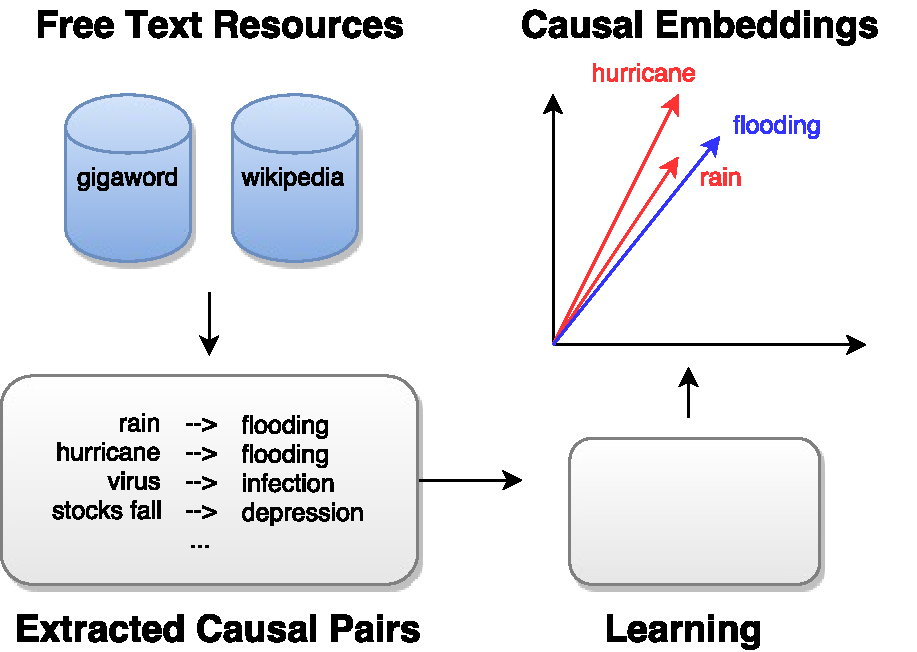
\includegraphics[width=75mm]{emnlpArchDraft.pdf}
%%\vspace{-4mm}
%\caption{{\small Our proposed pipeline for training a causal embedding space from free text resources. \todo{fill in learning with final model}}}
%\vspace{-6mm}
%\label{fig:arch}
%\end{center}
%\end{figure}
%
%\section{Approach}
%\label{sec-emnlp2016:approach}
%%\vspace{-2mm}
%
%Our focus is on reranking answers to causal questions using using task-specific distributional similarity methods.
%%on the the task of question answering, which is complicated by the variety of question types (e.g., definitional, causal),  each having different information needs that potentially require dedicated solving methods~\cite{clark2013study}.  
%%Longer term, we propose a QA approach which uses dedicated, task-specific word embeddings for each question type, aimed at maintaining the robustness of word embeddings while gaining the specificity of dedicated solving methods. 
%%Here, we address one particular information need: causality.
%%
%Our approach operates in three steps:
%
%{\flushleft (1)} We start by bootstrapping a large number of cause-effect pairs from free text using a small number of syntactic and surface patterns (Section \ref{sec-emnlp2016:causalextraction}).
%
%{\flushleft (2)} We then use these bootstrapped pairs to build several task-specific embedding (and other distributional similarity) models (Section \ref{sec-emnlp2016:models}). We evaluate these models directly on a causal-relation identification task (Section \ref{sec-emnlp2016:directeval}).  
%
%{\flushleft (3)} Finally, we incorporate these models into a reranking framework for causal QA and demonstrate that the resulting approach performs better than the reranker without these task-specific models, even if trained on the same data (Section ~\ref{sec-emnlp2016:indirecteval}).  


%We approach the task of creating and evaluating a task-specific relational vector space by considering one relation in particular -- causality.  The architecture of our system is shown in Figure \ref{fig:arch}. \todo{do I really need an architecture here?}

%rule-based framework which analyzes free text and returns cause-effect tuples.  
%These pairs are then used to learn a set of high-dimensional word embeddings which are particular to the desired relation.  
%In particular, we make use of the Levy and Goldberg extension of the skipgram algorithm to learn embeddings from these pairs by predicting the effect-text given the cause-text.
%MOVE:
%using the extension of the Skipgram algorithm~\todo{cite and link} proposed by \citep{levy2014dependency}.  
%\todo{does this belong here? intro?}
%While the learning algorithm returns two distinct vector space embeddings for each item in the vocabulary, often only the target embeddings are ever used.  In this work, however, we make use of both sets of embeddings to capture the inherent \emph{directionality} of the causal relation.

%\todo{remove the evaluation info from here?}
%Once trained, we then evaluate the quality this mapping, or vector space, in two ways.  First, we evaluate it directly by attempting to rank a set of cause-effect pairs higher than entity pairs from other relations.  Second, we evaluate the mapping indirectly, by using it in the down-stream task of question answering (QA).



\section{Extracting Cause-Effect Tuples}
\label{sec-emnlp2016:causalextraction}
%\vspace{-2mm}

%Information extraction (IE) systems which are designed to extract events typically make use of either machine learning (ML) or hand-built rules or patterns.  %IE classifiers which use ML are generally considered to be either fully supervised (trained only on annotated data), semi-supervised (trained on a combination of labelled data and the data which is bootstrapped from it or by using a large database of pre-known event tuples), or unsupervised (when no labelled data is available for training).
%For causal events, we have neither labelled data nor an existing, large database of cause-effect pairs from which we could use ML to train a supervised or semi-supervised classifier.  Additionally, while unsupervised or distant supervision approaches are well-suited to situations where the desired event types and the patterns that would identify them are unknown, here we know exactly what relation we want (causality) and the patterns needed to find these events are relatively explicit.  For these reasons, we opted to use boostrapping to extract a large number of cause-effect pairs from a small set of patterns.

Because the success of embedding models depends on large training datasets \citep{sharp-EtAl:2015:NAACL-HLT}, and such datasets do not exist for open-domain causality, we opted to bootstrap a large number of cause-effect pairs from a small set of patterns.
%
We wrote these patterns using Odin~\citep{valenzuela2016runes}, a rule-based information extraction framework which has the distinct advantage of 
%being able to operate over multiple representations of content (i.e., surface and syntax).
being \emph{expressive}.  That is, while most open-source rule languages operate over one representation of text (e.g., GATE~\citep{Cunningham2011a} generally operates over surface sequences, whereas Semgrex~\citep{chambers2007learning} operates over syntactic dependencies), Odin has the flexibility to use either (or both) depending on the user's need.  
For this work, we make use of rules that operate over both surface sequences as well as dependency syntax in the grammars introduced in steps (2) and (3) below.

Odin operates as a cascade, % of grammars, 
allowing us to implement a two-stage approach.
%. Taking advantage of this architecture, we implemented a two-stage approach.
First, we identify potential participants in causal relations, i.e., the potential causes and effects, which we term {\bf causal mentions}. A second grammar then identifies actual causal relations that take these causal mentions as arguments.

We consider both noun phrases (NP) as well as entire %non-causal
clauses to be potential causal mentions, since causal patterns form around participants that are syntactically more complex than flat NPs.  
%For example, in the sentence \emph{The hurricane caused significant damage}, both the cause ({\em hurricane}) and effect ({\em damage}) are non-recursive noun phrases.  On the other hand, 
For example, in the sentence \emph{The collapse of the housing bubble caused stock prices to fall}, both the cause ({\em the collapse of the housing bubble}) and effect ({\em stock prices to fall}) are more complicated nested structures.  Reducing these arguments to non-recursive NPs (e.g., {\em The collapse} and {\em stock prices}) is clearly insufficient to capture the relevant context.

Formally, we extract our causal relations using the following algorithm:
{\flushleft \textbf{(1) Pre-processing:}} Much of the text we use to extract causal relation tuples comes from the Annotated Gigaword \citep{napoles2012annotated}.  This text is already fully annotated and no further processing is necessary.  We additionally use text from the Simple English Wikipedia\footnote{{\scriptsize \url{https://simple.wikipedia.org/wiki/Main_Page}}.  The Simple English version was preferred over the full version due to its simpler sentence structures, which make extracting cause-effect tuples more straightforward.}, which we processed using the Stanford CoreNLP toolkit~\citep{Manning:14} and the dependency parser of \citet{chen14}.

{\flushleft \textbf{(2) Causal mention identification:}} \label{step:cm} We extract causal mentions (which are able to serve as arguments, i.e., the cause or effect,  in our causal patterns) using a set of rules (shown in Appendix \ref{appendix:cm_rules})\todo{rule appendix!} 
designed to be robust to the variety that exists in natural language. %, and therefore in the dependency parses.  
Namely, to find causal mentions that are noun phrases, we first find words that are tagged as nouns, then follow outgoing dependency links for modifiers and attached prepositional phrases\footnote{The outgoing dependency links from the nouns which we followed were: \texttt{nn, amod, advmod, ccmod, dobj, prep\_of, prep\_with, prep\_for, prep\_into, prep\_on, prep\_to}, and \texttt{prep\_in}.}, to a maximum depth of two links.  To find causal mentions that are clauses, we first find words that are tagged as verbs (excluding verbs which themselves were considered to signal causation\footnote{The verbs we excluded were: \emph{cause, result, lead, create}.}), then again follow outgoing dependency links for modifiers and arguments.  We used a total of four rules to label causal mentions.%\footnote{The two complete grammars, for both causal mention and causal relation identification, were submitted as supplemental material. \todo{This is no longer relevant. Please remove.}}
%There were a total of four rules used to label causal mentions, and examples are shown in Table~\ref{tab:rules}.

{\flushleft \textbf{(3) Causal tuple extraction:}} \label{step:causalext} After causal mentions are identified, a grammar scans the text for causal relations that have causal mentions as arguments.  Different patterns have varying probabilities of signaling causation~\citep{khoo1998automatic}.  To minimize the noise in the extracted pairs, we restrict ourselves to a set of 13 rules designed to find unambiguously causal patterns, such as {\em CAUSE led to EFFECT}, where {\em CAUSE} and {\em EFFECT} are previously found causal mentions.
The rules operate by looking for a \emph{trigger} phrase, e.g., {\em led}, and then following the dependency paths to and/or from the trigger phrase to see if all required causal mention arguments exist.
%, which tells the rule to fire.  Once a trigger is found, the rule follows the dependency paths to and/or from the trigger phrase to see if all specified arguments exist, e.g.,  following an outgoing {\tt nsubj} to identify the cause in the previous example.
%An example of this is shown in Figure \ref{fig:rule_ex}. Here, when the rule scans the sentence \emph{SENTENCE TEXT}, the trigger verb \emph{cause} is found, then the rule checks for an outgoing \texttt{nsubj} dependency link and an outgoing \texttt{dobj} link to previously found causal mentions.  
%%Our grammars also ensure that the triggers are not negated (we used Odin lookaround assertions to check that outgoing \texttt{neg} dependencies are not attached to triggers).  % Since in this example, all conditions are met, the rule returns the causal event in the form of the tuple (\todo{example}).

% ms: removed for space
At step~2, the identification of causal mentions, we place few restrictions on the causal mention syntactic subgraph, favoring recall since in step 3 we use high-precision rules.  The rule set for step \ref{step:causalext}, in fact, was winnowed down after early experiments showed that many patterns which \emph{can} indicate causation (e.g., {\em X happened due to Y}) often are non-causal.  

\begin{table}[t!]
\begin{center}
%\begin{scriptsize}
%\begin{footnotesize}
\begin{tabular}{lc}
\hline
Corpus		&	Extracted Tuples		 \\
\hline
%\multicolumn{2}{l}{\textit{Yahoo! Answers}} \\ % 185q (sent) ret=1p c=0.1 
%\hline
Annotated Gigaword	& 798,808 	\\
Simple English Wikipedia		& 16,425 	\\
\hline
Total		& 815,233 	\\
\end{tabular}
%\end{footnotesize}
\caption{{\footnotesize Number of causal tuples extracted from each corpus.}} 
\label{tab:causalstats}
%space{-4mm}
\end{center}
\end{table}

%ltw_mar30_combo.argsC: 55882
%nyt_mar30_combo.argsC: 260460
%wpb_mar30_combo.argsC: 7522
%apw_mar30_combo.argsC: 219348
%xin_mar30_combo.argsC: 76183
%simpleWiki_mar19b_combo.argsC: 14057
%cna_mar30_combo.argsC: 7913
%afp_mar30_combo.argsC: 133003
%sum: 774368

Applying this causal grammar over Gigaword and Simple English Wikipedia produced 815,233 causal tuples, as summarized in Table~\ref{tab:causalstats}. As bootstrapping methods are typically noisy, we manually evaluated the quality of approximately 250 of these pairs selected at random.  Of the tuples evaluated, approximately 44\% contained some amount of noise. For example, from the sentence 
\begin{quote}
\emph{Except for Springer's show, which still relies heavily on confrontational topics that lead to fistfights virtually every day...}
\end{quote}
%\emph{Except for Springer's show, which still relies heavily on confrontational topics that lead to fistfights virtually every day...}
while ideally we would only extract (\emph{confrontational topics $\rightarrow$ fistfights}), instead we extract the tuple (\emph{show which still relies heavily on confrontational topics} $\rightarrow$ \emph{fistfights virtually every day}), which contains a large amount of noise: \emph{show, relies, heavily}, etc.
This finding prompted our noise-aware model described at the end of Section~\ref{sec-emnlp2016:models}.


\section{Models}
\label{sec-emnlp2016:models}

We use the extracted causal tuples to train three distinct distributional similarity models that explicitly capture causality. 

{\flushleft \textbf{Causal Embedding Model (cEmbed):}}
The first distributional similarity model we use is based on the skip-gram word-embedding algorithm of Mikolov et al.~\citeyear{mikolov2013distributed}, which has been shown to improve a variety of language processing tasks % \footnote{Chris Manning recently called embedding models the Sriracha sauce of NLP.} 
including QA~\cite{yih13,fried2015higher}.  In particular, we use the variant implemented by Levy and Goldberg~\citeyear{levy2014dependency} which modifies the original algorithm to use an arbitrary, rather than linear, context. 
Our novel contribution is to make this context task-specific: intuitively, the context of a cause is its effect. Further, these contexts are generated from tuples that are themselves bootstrapped, which minimizes the amount of supervision necessary.

The Levy and Goldberg model trains using single-word pairs, while our CMs could be composed of multiple words.  
For this reason, we decompose each cause--effect tuple, $(CM_c,CM_e)$, such that each word $w_c \in CM_c$ is paired with each word $w_e \in CM_e$. 

%so we decompose each cause--effect tuple, $(CM_c,CM_e)$, where each CM could be multi-word, into the Cartesian product of the words in CMs. such that each $w_c \in CM_c$ has as its context all $w_e \in CM_e$. 
After filtering the extracted cause-effect tuples for stop words and retaining only nouns, verbs, and adjectives, we generated over 3.6M $(w_c, w_e)$ word-pairs\footnote{For all models proposed in this section we used lemmas rather than words.} from the approximately 800K causal tuples.

The model learns two embedding vectors for each word, one for when the word serves as a target word and another for when the word serves as a context word.  Here, since the relation of interest is inherently directional, both sets of embeddings are meaningful, and so we make use of both -- the target vectors encode the effects of given causes, whereas the context vectors capture the causes of the corresponding effects. 


{\flushleft \textbf{Causal Alignment Model (cAlign):}}
Monolingual alignment (or translation) models have been shown to be successful in QA \cite{Berger:00,Echihabi:03,Soricut:06,Riezler:etal:2007,Surdeanu:11,yao2013}, and recent work has shown that they can be successfully trained with less data than embedding models~\cite{sharp2015spinning}. 
% Further, Fried et al.~\citeyear{fried2015higher} demonstrated that \todo{dest. distribution as semantic model of the source concept, which is important for our task as well.} % ms: nice, but no space

To verify these observations in our context, we train an alignment model that ``translates'' causes (i.e., the ``source language'') into effects (i.e., the ``destination language''), using our cause--effect tuples. 
This is done using IBM Model 1~\cite{Brown:93} and GIZA++~\cite{och03}. 
%We train an alignment model from our cause--effect tuples using  IBM Model 1~\cite{Brown:93} and GIZA++~\cite{och03}.


\begin{figure}[t!]
\begin{center}
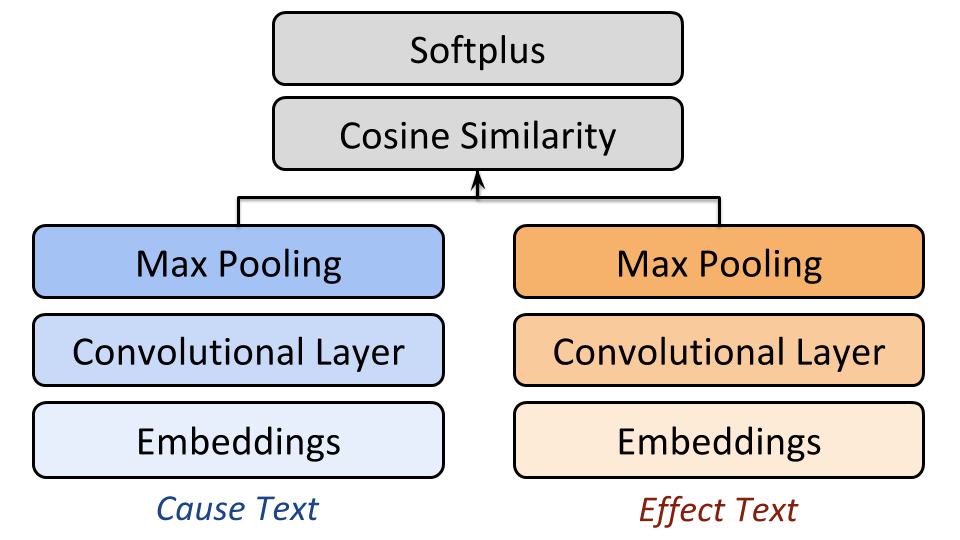
\includegraphics[width=0.7\textwidth]{mainmatter/emnlp2016-causal/cnn2.png}
%space{-2mm}
\caption{{\footnotesize Architecture of the causal convolutional network. }}
%space{-6mm}
\label{fig:cnn}
\end{center}
\end{figure}

{\flushleft \textbf{Causal Convolutional Neural Network Model (cCNN):}}
Each of the previous models have at their root a bag-of-words representation, which is a simplification of the causality task. To address this potential limitation, we additionally trained a convolutional neural network (CNN) which operates over variable-length texts, and maintains distinct embeddings for causes and effects.  The architecture of this approach is shown in Figure~\ref{fig:cnn}, and consists of two sub-networks (one for cause text and one for effect text), each of which begins by converting the corresponding text 
% (which has been padded to be of equal  length)  % ms: skip for now, until we understand it better
into 50-dimensional embeddings.  These are then fed to a convolutional layer,\footnote{The convolutional layer contained 100 filters, had a filter length of 2 (i.e., capturing bigram information), and an inner ReLU activation.} which is followed by a max-pooling layer of equal length.
Then, these top sub-network layers, which can be thought of as a type of phrasal embedding, are merged by taking their cosine similarity.  Finally, this cosine similarity is normalized by feeding it into a dense layer with a single node which has a softplus activation.  
In designing our CNN, we attempted to minimize architectural and hyperparameter tuning by taking inspiration from Iyyer et al.~\citeyear{iyyer2015deep}, preferring simpler architectures.
We train the network using a binary cross entropy objective function and the Adam optimizer~\cite{kingma2014adam}, using the Keras library~\cite{chollet2015keras} operating over Theano~\cite{2016arXiv160502688short}, a popular deep-learning framework.\footnote{We also experimented with an equivalent architecture where the sub-networks are implemented using long short-term memory (LSTM) networks~\cite{hochreiter1997long}, and found that they consistently under-perform this CNN architecture. Our conjecture is that CNNs perform better because LSTMs are more sensitive to overall word order than CNNs, which capture only local contexts, and we have relatively little training data, which prevents the LSTMs from generalizing well.}

{\flushleft \textbf{Noise-aware Causal Embedding Model (cEmbedNoise):}} 
We designed a variant of our cEmbed approach to address the potential impact of the noise introduced by our bootstrapping method.
While training, we weigh the causal tuples by the likelihood that they are truly causal, which we approximate with pointwise mutual information (PMI).
For this, we first score the tuples by their causal PMI and then scale these scores by the overall frequency of the tuple~\cite{riloff1996automatically}, to account for the PMI bias toward low-frequency items.  That is, the score $S$ of a tuple, $t$, is computed as: 

%space{-2mm}
%\scalebox{1.0}{
\begin{small}
\begin{equation}
S(t) = \log \frac{p(tuple|causal)}{p(tuple)} * \log (freq(tuple))
\end{equation} 
\end{small}
%}
%space{-2mm}

%Riloff~\citeyear{riloff1996automatically} propose a method for ranking their extracted patterns using $relevance\_rate * \log_2 (frequency)$.  As our relevance rate we use the pointwise mutual information of the extracted tuples, or $\log \frac{p(tuple|causal)}{p(tuple)}$, where $p(tuple| causal)$ is the ratio of the number of times that a given tuple is found in a causal construction versus any construction, and $p(tuple)$ is the frequency of the given tuple divided by the frequency of all the tuples. 
%Scaling the PMI by the frequency of the tuple mitigates its bias towards low-frequency items.
%we combine PMI with frequency information, so that we consider the likelihood of a pair to be causal to be:
%$p(causal|pair)$ \cite{riloff1996automatically}.
We then discretize these scores into five quantiles, ascribing a linearly decreasing weight during training to datums in lower scoring quantiles.%\footnote{\textcolor{blue}{We implemented this weighing process by repeating higher weight training examples more times.}}



\section{Direct Evaluation: Ranking Word Pairs}

\begin{figure*}[th!]
\begin{center}
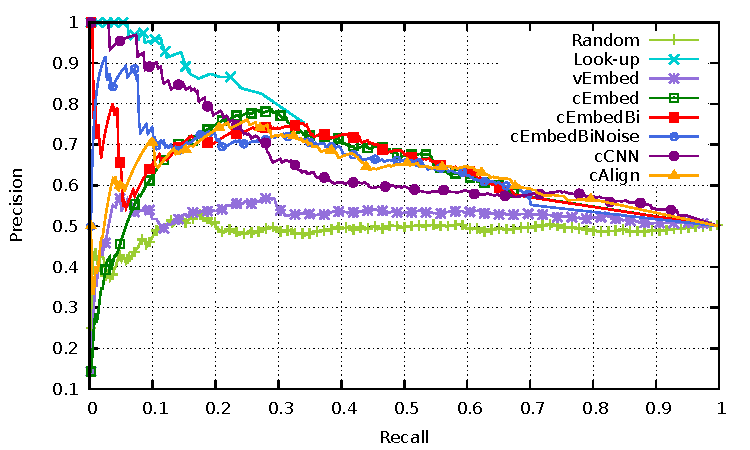
\includegraphics[width=\textwidth]{mainmatter/emnlp2016-causal/direct2.pdf} % {rpcurves_all.png}
%space{-3mm}
\caption{{\footnotesize Precision-recall curve showing the ability of each model to rank causal pairs above non-causal pairs. For clarity, we do not plot cEmbedNoise, which performs worse than cEmbedBiNoise. The Look-up model has no data points beyond the 35\% recall point.}}
%space{-4mm}
\label{fig:rpcurve_all}
\end{center}
\end{figure*}

%\flushleft{\textbf{Results:}} 

\label{sec-emnlp2016:directeval}

%Before we discuss the utility of these models for causal QA, we implement a {\em direct} evaluation
We begin the assessment of our models with a {\em direct} evaluation to determine whether or not the proposed approaches capture causality better than general-purpose word embeddings and whether their robustness improves upon a simple database look-up.
For this evaluation, we follow the protocol of Levy and Goldberg~\citeyear{levy2014dependency}.  
In particular, we create a collection of word pairs, half of which are causally related, with the other half consisting of other relations. 
These pairs are then ranked by our models and several baselines, with the goal of ranking the causal pairs above the others. 
The embedding models rank the pairs using the cosine similarity between the target vector for the causal word and the context vector of the effect word.  The alignment model ranks pairs using the probability $P(\text{Effect}|\text{Cause})$ given by IBM Model 1, and the CNN ranks pairs by the value of the output returned by the network.
%To demonstrate that their embeddings encoded functional similarity rather than relatedness, they ranked a set of word pairs (each of which reflected one of the two types of similarity) using cosine similarity and showed that the word pairs which were functionally similar tended to be ranked higher than those with topical similarity.  Here, we do the same.

%\flushleft{\textbf{Data:}} 
\subsection{Data}
In order to avoid bias towards our extraction methods, we evaluate our models on an external set of word pairs drawn from the SemEval 2010 Task 8 \cite{hendrickx2009semeval}, originally a multi-way classification of semantic relations between nominals.  We used a total of 1730 nominal pairs, 865 of which were from the Cause-Effect relation (e.g., (\emph{dancing $\rightarrow$ happiness})) and an equal number which were randomly selected from the other eight relations (e.g., (\emph{juice $\rightarrow$ grapefruit}), from the Entity-Origin relation).  This set was then randomly divided into equally-sized development and test partitions.

%\flushleft{\textbf{Baselines:}} 
\subsection{Baselines}
We compared our distributional similarity models against three baselines:

{\flushleft \textbf{Vanilla Embeddings Model (vEmbed):}} a standard \texttt{word2vec} model trained with the skip-gram algorithm and a sliding window of 5, using the original texts from which our causal pairs were extracted.\footnote{All embedding models analyzed here, including this baseline and our causal variants, produced embedding vectors of 200 dimensions.} As with the cEmbed model, SemEval pairs were ranked using the cosine similarity between the vector representations of their arguments.
%space{-1mm}

{\flushleft \textbf{Look-up Baseline:}} a given SemEval pair was ranked by the number of times it appeared in our extracted cause-effect tuples. 
%space{-1mm}

{\flushleft \textbf{Random:}} pairs were randomly shuffled.
%space{-1mm}



%%
%% MAP Table 
%%
%\begin{table}[t!]
%\begin{center}
%%\begin{scriptsize}
%\begin{footnotesize}
%\begin{tabular}{ll}
%\hline
%\multicolumn{1}{l}{ Model } & \multicolumn{1}{l}{MAP} \\ %\multicolumn{1}{l}{Impr.} \\
%%\cline{1-2}
%\hline
%%\multicolumn{2}{l}{\textit{Yahoo! Answers}} \\ % 185q (sent) ret=1p c=0.1 
%%\hline
%Random 			& 48.8 	\\
%Look-up			& 63.1$^*$ 	\\
%vEmbed 			& 52.5	\\
%cEmbed  			& 60.8$^*$	\\
%cEmbedBi	                & 62.8$^*$	\\
%cEmbedNoise           & 62.0$^*$	\\ 
%cEmbedBiNoise        & 63.6$^*$	\\ 
%cAlign  			& 61.6$^*$  \\
%cCNN  			& 67.5$^*$	\\
%\end{tabular}
%\end{footnotesize}
%\caption{{\footnotesize Performance in the direct evaluation, measured with mean average precision (MAP).  The ``Bi'' suffix indicates a bidirectional model; the ``Noise'' suffix indicates a model that is noise aware. $^*$  indicates that the difference between the corresponding model and vEmbed is statistically significant ($p < 0.05$), %. Statistical significance was 
%as determined through a one-tailed bootstrap resampling test with 10,000 iterations.}} 
%\label{tab:MAP}
%\vspace{-4mm}
%\end{center}
%\end{table}
%%MAP for Custom Vectors: 0.6816675505751166
%%MAP for E2C Vectors: 0.6871338630607531
%%MAP for Bidir Vectors: 0.6684350003582593
%%MAP for Comparison (Baseline) Vectors: 0.5835158858435683
%%MAP for Translation Model with lamda of 0.5 : 0.6156522257806402
%%MAP for counting Matches: 0.9312613087523468
%%MAP for Keras: 0.6752727545259546
%%MAP for Random: 0.4892479543525109
%%p < 0.01


\subsection{Results}

Figure \ref{fig:rpcurve_all} shows the precision-recall (PR) curve for each of the models and baselines. 
As expected, the causal models are better able to rank causal pairs than the vanilla embedding baseline (vEmbed), which, in turn, outperforms the random baseline.  Our look-up baseline, which ranks pairs by their frequency in our causal database, shows a high precision for this task, but has coverage for only 35\% of the causal SemEval pairs.
%This demonstrates that it is beneficial to have custom models for the semantic relation of interest. 
%First, all the proposed models perform better than the vanilla embedding baseline (vEmbed), which, in turn, outperforms the random baseline. 
%The difference between all our proposed causal models and the vEmbed baseline is statistically significant. 
%

Some models perform better on the low-recall portion of the curve (e.g., the look-up baseline and cCNN), while the embedding and alignment models have a higher and more consistent performance across the PR curve. We hypothesize that models that better \emph{balance} precision and recall will perform better in a real-world QA task, which may need to access a given causal relation through a variety of lexical patterns or variations. We empirically validate this observation in Section~\ref{sec-emnlp2016:indirecteval}.

%, suggesting that causal embedding models may be more practical in a real-world QA system than cCNN. We empirically validate this intuition in Section. 

%perform better in the mid-low recall portion of the curve (e.g. cEmbedBi).  This is well-illustrated by the look-up baseline, which has high precision in the low-recall portion of the curve, but which only has coverage of 35\% of the causal SemEval pairs.  
%The cCNN model outperforms the cEmbed and cAlign models for the low-recall part of the curve (which explains why cCNN has the highest overall MAP). But the latter models 


%Second, the look-up baseline has a higher MAP than several of the causal models, despite having coverage of only 35\% of the causal SemEval pairs.  This suggests that the MAP score is dominated by precision, rather than recall.
%Despite the high overall MAP, this lack of coverage renders this an impractical model, because a real-world QA system is more likely to encounter questions that are lexically different than the pairs in our database. 


%Second, we see that models which had higher MAP demonstrate higher precision in the low-recall portion of the curve, while the models which perform better in the mid-low recall portion of the curve have slightly lower MAPs.  
%This is well-illustrated by the Look-up baseline, whose MAP is higher than many of the causal models, and which has excellent precision in the low-recall portion of the curve, but which only provides coverage for 35\% of the causal pairs.  
%We hypothesize that is the models that better balance precision and recall that will perform well in a real-world QA system, where it is more likely that questions will be lexically different than the pairs in our database.


%Second, somewhat disturbingly, the look-up baseline seemingly outperforms most of the embedding models. 

%However, this score is highly skewed by the fact that approximately 35\% of the causal SemEval pairs were also found in our casual database, and were scored with high precision due to the direct evidence available. However, the remaining pairs received a score of 0. 

%% WHAT IT JUST WAS:
%However, this score is highly skewed: 35\% of the causal SemEval pairs were also found in our casual database, and so were scored with high precision due to the direct evidence available, but the remaining 65\% of pairs all received a score of 0.
%Despite the high overall MAP, this lack of coverage renders this an impractical model, because a real-world QA system is more likely to encounter questions that are lexically different than the pairs in our database. 

%Thus, the MAP score for this model is unrealistically skewed.
% \todo{Say something about how these evaluations are not ideal}~\cite{faruqui2016problems}.

%the high precision of pairs which are found in the database coupled with the very low recall (only 35\% of the pairs were found in the extracted pairs), resulting in the majority of the pairs being tied in the lowest rank, skewing the average.
%that when pairs are found, there is extremely high confidence that they are of the relation of interest coupled with the fact that approximately 65\% of the pairs were not found in the database and so were all tied in last place.  
%As a consequence, there were far fewer average precisions to be combined when calculating the MAP, and most of the ones which were there had extremely high precision.  
% The MAP when using the customized vectors was significantly higher than that of the standard \texttt{word2vec} vectors (68\% versus 58\%, $p<0.01$), and both were higher than the baseline ().  %This suggests that while the standard implementation of \texttt{word2vec} encodes some causality information, our method encodes it far more directly. \todo{better word}.

% \subsection{Discussion}
%To better understand these models, we plot the precision-recall (PR) curve in Figure \ref{fig:rpcurve_all}. 
%The curve highlights the issue discussed above: the look-up model ranks a few pairs with high precision, but does not address the majority of the data. 
%Conversely, the proposed causal models consistently outperform the vEmbed baseline for the high-recall portion of the curve.



The PR curve for the causal embeddings shows an atypical dip at low-recall.  To examine this, we analyzed its top-ranked 15\% of SemEval pairs, and found that incorrectly ranked pairs were not found in the database of causal tuples.  Instead, these incorrect rankings were largely driven by low frequency words whose embeddings could not be robustly estimated due to lack of direct evidence.  
%\todo{Optional: I know we're low on space, but the example that Becky had here was great. Any way to put it back?}
Because this sparsity is partially driven by directionality, 
we implemented a bidirectional embedding model (cEmbedBi) that (a) trains a second embedding model by reversing the input (effects as targets, causes as contexts), and (b) ranks pairs by the \textit{average} of the scores returned by these two unidirectional causal embedding models. 
Specifically, the final bidirectional score of the pair, $(e_1, e_2)$, where $e_1$ is the candidate cause and $e_2$ is the candidate effect, is:
\begin{equation}
s_{bi}(e_1, e_2) = \tfrac{1}{2}(s_{c{\rightarrow}e}(e_1, e_2) + s_{e \rightarrow c}(e_2, e_1))
\end{equation}
where $s_{c \rightarrow e}$ is the score given by the original causal embeddings, i.e., from cause to effect, and $s_{e \rightarrow c}$ is the score given by the reversed-input causal embeddings, i.e., from effect to cause.

As Figure~\ref{fig:rpcurve_all} shows, the bidirectional embedding variants consistently outperform their unidirectional counterparts. 
All in all, the best overall model is cEmbedBiNoise, which is both bidirectional and incorporates the noise handling approach from Section~\ref{sec-emnlp2016:models}. This model substantially improves performance in the low-recall portion of the curve, while also showing strong performance across the curve. 



%
%The curve for the customized vectors shows an atypical shape in its low-recall part.
%Here, the highest ranked pairs had \emph{worse} precision rather than the expected higher precision.  To examine this, we analyzed the top-ranked 15\% of the pairs from the ranking produced by  the causal vectors.  
%%
%Our analysis found that these pairs tend to be incorrectly ranked because the cEmbed model performs a form of soft approximate inference (which was our goal!), but which backfired on these data points.  For example, the top-ranked (incorrect) pair was \emph{platform} $\rightarrow$ \emph{scaffold}, and there were no instances in our causal database where \emph{platform} and \emph{scaffold} were found together in the same cause-effect pair.  
%%
%Instead, we found that there were  three other extracted tuples with \emph{scaffold} in the effect text. Further, these tuples had other effects  that overlapped lexically with effects of \emph{platform}, which ``pulled'' \emph{platform} closer to \emph{scaffold}.  For example, a phrase containing \emph{malfunction} 
%shares {\em loss} as a common effect with \emph{platform}, and \emph{malfunction} has other effects that contain \emph{scaffold}. 
%In general, we found that these examples of semantic drift~\cite{curran2007minimising} occur for low frequency data, where neither the direct evidence nor the embeddings are robustly estimated. 
%
%%cause \emph{loss}, which brings these two words closer in the target embedding space.
%%%, since they have similar effects.  
%%This resulted in \emph{platform}'s effects being close to the effects of \emph{malfunction}, which include \emph{scaffold}.  This demonstrates that the inference is influenced by frequency effects, as words like \emph{scaffold} and \emph{platform} are too infrequent to have robust representations in the embedding space.  
%%\todo{This last sentence needs better explanation: why does this happen only at low-recall?}
%
%As this semantic drift effect is entirely directional, we implemented a bidirectional embedding approach, which: (a) trains a second embedding model by reversing the input, such that the effects served as the targets and the causes were the contexts, and (b) 
%ranks pairs by the average of the scores returned by the two causal embeddings. As Table~\ref{tab:MAP} and Figure~\ref{fig:rpcurve_all} show, the bidirectional embedding variants consistently outperform their unidirectional counterparts. cEmbedBiNoise, which incorporates the noise handling approach from Section~\ref{sec-emnlp2016:models} and is bidirectional, resolves the dip in low-recall part of the curve, and outperforms cCNN for most of the data. 
%
%%As this effect is entirely directional, we trained a set of vectors by reversing the input, such that the effects served as the targets and the causes were the contexts.  The precision-recall curve when using these embeddings to rank the SemEval pairs is shown in Figure \ref{fig:rpcurve_all}, labelled as E2C.  As expected, the curve follows that of the original vectors, as it suffers from the same issues, but with different noisy pairs ranked highly.  We then ranked the SemEval pairs using an average of the scores returned by the two causal embeddings, to mitigate the frequency effects.  That final, bidirectional curve is also shown in Figure \ref{fig:rpcurve_all}.
%%Instead, we found that many of the causal events which whose cause argument contained the word \emph{platform} had effects which overlapped lexically with those whose cause arguments contained the word \emph{malfunction}, and that there w.  To illustrate, consider the following sentences 
%%we had several extracted causal events whose cause contained the word \emph{platform} and whose effect contained the words \emph{}
%


%space{-1mm}
\section{Indirect Evaluation: QA Task}
%space{-1mm}
%\label{sec-emnlp2016:qa}
\label{sec-emnlp2016:indirecteval}

%\todo{Describe the QA system and its features shortly, in 1 paragraph.}
The main objective of our work is to investigate the impact of a customized causal embedding model for question answering (QA). Following our direct evaluation, which solely evaluated the degree to which our models directly encode causality, here we evaluate each of our proposed causal models in terms of their contribution to a downstream real-world QA task.

Our QA system here uses the same standard reranking approach~\citep{jansen14} as in Chapter \ref{chapter:naacl2015}.
In this architecture, the candidate answers are initially extracted and ranked using a shallow information retrieval (IR) component, then they are re-ranked using a ``learning to rank'' approach (see Section \ref{sec-naacl2015:models} for more details on the IR component and resulting IR score).
In particular, we used SVM rank\footnote{ \url{http://www.cs.cornell.edu/people/tj/svm_light/svm_rank.html}}, a Support Vector Machines classifier adapted for ranking, and re-ranked the candidate answers with a set of features derived from both the initial IR score and the models we have introduced. For our model combinations (see Table \ref{tab:QA}), the feature set includes the IR score and the features from each of the models in the combination.
%We compare the performance of our causal models against the same vanilla embeddings model (vEmbed) used in Section \ref{sec-emnlp2016:directeval}, the vanilla alignment model (vAlign) of Fried et al.~\citeyear{fried2015higher} trained over the same corpus as the questions,  as well as the look-up baseline.
%

\subsection{Data}

% Our models were trained on open-domain resources, so 
We evaluate on a set of causal questions extracted from the Yahoo! Answers corpus\footnote{Freely available through Yahoo!'s Webscope
program ({\scriptsize {\tt research-data-requests@yahoo-inc.com}})} with simple surface patterns such as \emph{What causes ...} and ~\emph{What is the result of ...}\footnote{We lightly filtered these with stop words to remove non-causal questions, such as those based on math problems and the results of sporting events. Our dataset is freely available, conditioned on users having obtained the Webscope license.}.
We extracted a total of 3031 questions, each with at least four candidate answers, and we evaluated performance using five-fold cross-validation, with three folds for training, one for development, and one for testing. 

\subsection{Models and Features}

We evaluate the contribution of the bidirectional and noise-aware causal embedding models (cEmbedBi, and cEmbedBiNoise) as well as the causal alignment model (cAlign) and the causal convolutional neural network (cCNN).  These models are compared against three baselines: the vanilla embeddings (vEmbed), the lookup baseline (LU), and additionally a vanilla alignment model (vAlign) which is trained over 65k question-answer pairs from Yahoo! Answers.

The features\footnote{Due to the variety of features used, each feature described here is independently normalized to lie between 0.0 and 1.0.} we use for the various models are:

{ \flushleft \textbf{Embedding model features:}}
For both our vanilla and causal embedding models, we use the same set of features as in Section \ref{sec-naacl2015:models} \citep{fried2015higher}: the maximum, minimum, and average pairwise cosine similarity between question and answer words, as well as the overall similarity between the composite question and answer vectors.  
When using the causal embeddings, since the relation is directed, we first determine whether the question text is the cause or the effect\footnote{We do this through with simple regular expressions, \mbox{e.g., ``\^~[Ww]hat ([a-z]+ )\{0,3\}cause.+''}}, which in turn determines which embeddings to use for the question text and which to use for the candidate answer texts.  For example, in a question such as "\emph{What causes X?}", since \emph{X} is the effect, all cosine similarities would be found using the effect vectors for the question words and the cause vectors for the answer candidate words. 

{\flushleft \textbf{Alignment model features:}} Again, as in Section \ref{sec-naacl2015:models}, we use the same global alignment probability, $p(Q|A)$ of \citet{Surdeanu:11}. In our causal alignment model, we adapt this to causality as $p(\text{Effect}|\text{Cause})$, and again we first determine the direction of the causal relation implied in the question.  We once again include the additional undirected alignment features based on Jensen-Shannon distance, proposed more recently by \citet{fried2015higher}, in our vanilla alignment model.  However, due to the directionality inherent in causality, they do not apply to our causal model so there we omit them.

{\flushleft \textbf{Look-up feature:}} For the look-up baseline we count the number of times words from the question and answer appear together in our database of extracted causal pairs, once again after determining the directionality of the questions.  If the total number of matches is over a threshold\footnote{Empirically determined to be 100 matches.  Note that using this threshold performed better than simply using the total number of matches.}, we consider the causal relation to be established and give the candidate answer a score of 1; or a score of 0, otherwise.

%\section{Downstream QA Evaluation}
%\label{sec-emnlp2016:indirecteval}

%The main objective of our work is to investigate the impact of problem-specific solving components for QA. 
%Here we focus on causal QA.
% develop dedicated question-answering (QA) system components for specific question types.  We therefore evaluate our causal models, which we previously determined to encode causality (Section \ref{sec-emnlp2016:indirecteval}), in a down-stream (QA) task with causal questions. 


\begin{table}[t!]
\begin{center}
%\begin{footnotesize}
\begin{footnotesize}
\begin{tabular}{lll}
\hline
\# & Model & P@1 \\ 
\hline
& Baselines & \\
\hline
1	&	Random 				& 16.43 	\\
2	&	CR					& 24.31	\\
3	&	CR + vEmbed 			& 34.61	\\
4	&	CR + vAlign			& 19.24	\\
5	&	CR + Look-up	 (LU)	& 29.56 	\\
\hline
& Single Causal Models 		& \\
\hline
6	&	CR + cEmbedBi       & 31.32\\
7	&	CR + cEmbedBiNoise  & 30.15 \\ 
8	&	CR + cAlign  		& 23.49 \\
9	&	CR + cCNN  			& 24.66	\\
\hline
& Model Combinations & \\
\hline
10	&	CR + vEmbed + cEmbedBi		& 37.08$^{*}$	\\ %p < 0.001
11	& 	CR + vEmbed + cEmbedBiNoise 	& 35.50$^*$	\\ %p < 0.05
12	&	CR + vEmbed + cEmbedBi + LU	& 36.75$^{*}$	\\ %p < 0.001
13	&	CR + vEmbed + cAlign		& 	34.31 	\\ %if worse, we can remove and just say that it doesn't stack, per Mihai
14	&	CR + vEmbed + cCNN		& 	33.45 \\
\hline
& Model Stacking & \\
\hline
%15	&	CR + vEmbed + cEmbedBi + cEmbedBi$^2$	& 37.22	\\
15	& 	CR + vEmbed + cEmbedBi + cEmbedBiNoise 	& {\bf 37.28$^{*}$}	\\ 

\end{tabular}
\end{footnotesize}
%space{-1mm}
\caption{{\footnotesize Performance in the QA evaluation, measured by precision-at-one (P@1).  The ``Bi'' suffix indicates a bidirectional model; the ``Noise'' suffix indicates a model that is noise aware. $^*$  indicates that the difference between the corresponding model and the CR + vEmbed baseline is statistically significant ($p < 0.05$), %. Statistical significance was 
determined through a one-tailed bootstrap resampling test with 10,000 iterations. }} 
\label{tab:QA}
%space{-8mm}
\end{center}
\end{table}

\subsection{Results}
The overall results are summarized in Table~\ref{tab:QA}.
Lines 1--5 in the table show that each of our baselines performed better than CR by itself, except for vAlign, suggesting that the vanilla alignment model does not generate accurate predictions for causal questions.
The strongest baseline was CR + vEmbed (line 3), the vanilla embeddings trained over Gigaword, at 34.6\% P@1. For this reason, we consider this to be the baseline to ``beat'', and perform statistical significance of all proposed models with respect to it. 

Individually, the cEmbedBi model is the best performing of the causal models.  While the performance of cAlign in the direct evaluation was comparable to that of cEmbedBi, here it performs far worse (line 6 vs 8), suggesting that the robustness of embeddings is helpful in QA.  Notably, despite the strong performance of the cCNN in the low-recall portion of the PR curve in the direct evaluation, here the model performs poorly (line 9).

No individual causal model outperforms the strong vanilla embedding baseline (line 3), likely owing to the reduction in generality inherent to building task-specific QA models.
However, comparing lines 6--9 vs. 10--14 shows that the vanilla and causal models are capturing different and complementary kinds of knowledge (i.e., causality vs. association through distributional similarity), and are able to be combined to increase overall task performance (lines 10--12).  These results highlight that QA is a complex task, where solving methods need to address the many distinct information needs in question sets, including both causal and direct association relations.  This contrasts with the direct evaluation, which focuses strictly on causality, and where the vanilla embedding baseline performs near chance. This observation highlights one weakness of word similarity tasks: their narrow focus may not directly translate to estimating their utility in real-world NLP applications. % \footnote{Continuing the food analogies initiated by Chris Manning, the direct evaluation is the equivalent of taking vitamin C instead of eating the whole orange (the downstream task).}

%Of the causal models, the highest performing was cEmbedBi, the bidirectional causal embedding model.  
%Additionally, we see that both of the causal embeddings models stack with the vEmbed model (lines 10 and 11).  
Adding in the lookup baseline (LU) to the best-performing causal model does not improve performance (compare lines 10 and 12), suggesting that the bidirectional causal embeddings subsume the contribution of the LU model.  
cEmbedBi (line 10) also performs better than cEmbedBiNoise (line 11). We conjecture that the ``noise'' filtered out by cEmbedBiNoise contains distributional similarity information, which is useful for the QA task.  cEmbedBi vastly outperforms cCNN (line 14), suggesting that strong overall performance across the precision-recall curve better translates to the QA task.  We hypothesize that the low cCNN performance is caused by insufficient training data, preventing the CNN architecture from generalizing well. 

%We see a small increase when we combine both variants of the causal embeddings model (cEmbedBi and cEmbedBiNoise -- line 15), showing that they contribute slightly different information. 
Our best performing overall model combines both variants of the causal embedding model (cEmbedBi and cEmbedBiNoise), reaching a P@1 of 37.3\%, which shows a 7.7\% relative improvement over the strong CR + vEmbed baseline.

% ms: replaced with text above
%Additionally, on the simpler direct evaluation, where the task consisted entirely of determining causality between two words, the causal models were superior to the baselines and seemingly more sufficient for the task.  The QA task, however, is more complex and not purely about determining causality.  Here we need both similarity \emph{and} causality to do well, as demonstrated by the significant improvement gained by stacking the cEmbed model with the vEmbed model.

% this is future work: I propose to skip it due to lack of space? Also, one of our main contribution is that this knowledge acquisition process is implemented independently of the evaluations. This paragraph negates that.
%\todo{discuss the noise variant and its lack of better performance}
%The failure of the noise-aware causal embeddings model to do better on the QA task suggests that the method we employed is not sufficient to the task.  For example, by weighing some examples more highly than others, we are not actually \emph{removing} the noise, only hoping to downplay it.  Additionally, the manner by which we weighed the extracted tuples was entirely disconnected from the training process as well as the down-stream task.  We suspect that learning the quality of the tuples jointly during training~\cite{tibshirani2014robust} might result in more robust task-specific noise-handling.


%\begin{table}[t!]
%\begin{center}
%%\begin{footnotesize}
%\begin{footnotesize}
%\begin{tabular}{ll}
%\hline
%Feature 	& SVM weight \\
%\hline
%CR	&	\\
%vEmbed max similarity		&	0.021\\
%cEmbed max similarity		&	0.828\\
%vEmbed min similarity		&	-1.703\\
%cEmbed min similarity		&	-0.445\\
%vEmbed avg similarity		&	-1.842\\
%cEmbed avg similarity		&	-2.177\\
%vEmbed overall similarity	&	2.867\\
%cEmbed overall similarity	&	1.725\\
%
%\end{tabular}
%\end{footnotesize}
%
%\caption{{\footnotesize SVM weights learned for each of the features in . }} 
%\label{tab:weights}
%\vspace{-8mm}
%\end{center}
%\end{table}

\begin{table}[t!]
\begin{center}
%\begin{footnotesize}
\begin{footnotesize}
\begin{tabular}{ll}
\hline
Error/observation 	& \% Q \\
\hline
Both chosen and gold are equally good answers 	& 	45\% \\ 
%Chosen answer is longer 							&	35\% \\
Causal max similarity of chosen is higher		&	35\% \\
Vanilla overall similarity of chosen is higher	&	35\% \\
Chosen answer is better than the gold answer		&	25\% \\
The question is very short / lacks content words	&	15\%	 \\
Other 											&	10\% \\
\end{tabular}
\end{footnotesize}

\caption{{\footnotesize Results of an error analysis performed on a random sample of 20 incorrectly answered questions showing the source of the error and the percentage of questions that were affected. Note that questions can belong to multiple categories. }} 
\label{tab:ea}
%space{-8mm}
\end{center}
\end{table}


\subsection{Error Analysis}
\label{sec-emnlp2016:erroranalysis}

We performed an error analysis to gain more insight into our model as well as the source of the remaining errors.  For simplicity, we used the combination model CR + vEmbed + cEmbedBi. Examining the model's learned feature weights, we found that the vanilla overall similarity feature had the highest weight, followed by the causal overall similarity and causal maximum similarity features.  This indicates that even in causal question answering, the overall \emph{topical} similarity between question and answer is still useful and complementary to the causal similarity features.


To determine sources of error, we randomly selected 20 questions that were incorrectly answered and analyzed them according to the categories shown in Table \ref{tab:ea}.  We found that for 70\% of the questions, the answer chosen by our system was as good as or better than the gold answer, often the case with community question answering datasets.


Additionally, while the maximum causal similarity feature is useful, it can be misleading due to embedding noise, low-frequency words, and even the bag-of-words nature of the model (35\% of the incorrect questions).  For example, in the question \emph{What are the effects of growing up with an older sibling who is better than you at everything?}, the model chose the answer \emph{...You are you and they are them - you will be better and different at other things...}  largely because of the high causal similarity between (\emph{grow} $\rightarrow$ \emph{better}).  While this could arguably be helpful in another context, here it is irrelevant, suggesting that in the future improvement could come from models that better incorporate textual dependencies.







%\vspace{-1mm}
\section{Conclusions}
\label{sec-emnlp2016:conclusion}
%\vspace{-1mm}
We presented a framework for creating customized embeddings tailored to the information need of causal questions.  We trained three popular models (embedding, alignment, and CNN) using causal tuples extracted with minimal supervision by bootstrapping cause-effect pairs from free text, and evaluated their performance both directly (i.e., the degree to which they capture causality), and indirectly (i.e., their real-world utility on a high-level question answering task).\footnote{All code and resources needed to reproduce this work are  available at \url{http://clulab.cs.arizona.edu/data/emnlp2016-causal/}.} 


%We note that the results of these two evaluations are not identical; higher performance on the direct evaluation does \emph{not} necessarily correlate with higher performance in the QA task.
We showed that models that incorporate a knowledge of causality perform best for both tasks. 
Our analysis suggests that the models that perform best in the real-world QA task are those that have consistent performance across the precision-recall curve in the direct evaluation.
In QA, where the vocabulary is much larger, precision must be balanced with high-recall, and this is best achieved by our causal embedding model.  Additionally, we showed that vanilla and causal embedding models address different information needs of questions, and can be combined to improve performance. 

Extending this work beyond causality, we hypothesize that additional embedding spaces customized to the different information needs of questions would allow for robust performance over a larger variety of questions, and that these customized embedding models should be evaluated both directly and indirectly to accurately characterize their performance. 

Despite the robustness of this model, and the extensibility to other question types, this model does not particularly provide interpretability.  This is demonstrated in the error analysis of Section \ref{sec-emnlp2016:erroranalysis} -- as the only outputs of the model are feature values and learned feature weights, it's difficult to explain to a human user (particularly a user who isn't well-versed in machine learning) why the system is choosing the answers it is.  This is addressed in Chapters \ref{chapter:cl2017} and \ref{chapter:emnlp2017} which follow, as each of these systems return a human-readable justification alongside the chosen answer to provide insight into what the model deems useful in determining a correct answer.

%We introduced a methodology for producing causal embedding models cost-effectively by bootstrapping cause-effect pairs extracted from free text using a small set of seed patterns, and then training dedicated embedding models over this data using task-specific contexts, i.e., where the context of a cause is its effect. We then used these causal embedding models to implement a dedicated reranking model for causal QA. 

%We evaluated the generated embedding models both directly, in a word similarity task, and indirectly, in the downstream QA task. Our analysis yielded multiple observations. First, causal embeddings significantly outperform vanilla embeddings in both tasks, demonstrating the importance of having dedicated models for the task at hand. Second, for QA, the causal embeddings stack well with vanilla ones, highlighting that QA is a complex task, where solving methods need to address multiple information needs. Third, we note that the results of these two evaluations are not identical; higher performance on the direct evaluation does not necessarily correlate with higher performance in the QA task. Our analysis suggests that the performance on the direct evaluation is driven by precision, whereas for the real-world QA task, where the vocabulary is much larger, the precision must be balanced with high-recall which is best achieved by our causal embedding model.  

%We hypothesize that additional embedding spaces customized to the different information needs of questions would allow for robust performance over a larger variety of questions, and that these customized embedding models should be evaluated both directly and indirectly to accurately characterize their performance. 


% ms: removed for anonymous submission
%\section*{Acknowledgments}
%We thank the Allen Institute for Artificial Intelligence for funding this work.
%Additionally, this work was partially funded by the Defense Advanced
%Research Projects Agency (DARPA) Big Mechanism
%program under ARO contract W911NF-14-1-0395.


\newpage
%\bibliography{emnlp2016}
%\bibliographystyle{emnlp2016}

%\end{document}
